% SC2203 --- Chapter 1: Alphabets, Strings, Languages (0->100 ground-up)
\chapter{Alphabets, Strings and Languages}
\label{ch:alphabets}

\begin{quote}
\emph{``What is a language, formally?''} --- Before automata can recognise anything, we need a precise universe: symbols strung into words, words collected into languages, and operations that build new languages from old.
\end{quote}

\noindent\fbox{\parbox{\dimexpr\linewidth-2\fboxsep-2\fboxrule}{%
\textbf{From zero: we build here, no prior theory needed.} We assume only sets and functions. Every notion---alphabet, string, language, Kleene star---is motivated by a picture, then defined, then exercised. No automata, grammars, or computability is assumed.}}
\vspace{0.4em}

\section*{Learning Outcomes}
After this chapter you will be able to:
\begin{enumerate}[label=(L\arabic*)]
    \item define alphabet, string, empty string and length, and count strings over an alphabet;
    \item distinguish string operations (concatenation, reversal, substring) and prove their basic laws;
    \item define language as a set of strings and apply Boolean and concatenation operations to languages;
    \item define Kleene star, plus, and closure properties, and compute small examples;
    \item recognise lexicographic and shortlex orderings and prove elementary cardinality results.
\end{enumerate}

% ============================================================
\section{Alphabets and Strings}
\label{sec:alphabets}
A \emph{symbol} is an indivisible mark---\texttt{a}, \texttt{0}, $\#$. An \emph{alphabet} $\Sigma$ is a finite non-empty set of symbols. Examples: $\Sigma=\{0,1\}$ (binary), $\Sigma=\{a,b,\dots,z\}$, $\Sigma=\{\texttt{a},\texttt{b}\}$.

% TikZ 1: alphabet as box of symbols -> strings as rows
\begin{figure}[h]
\centering
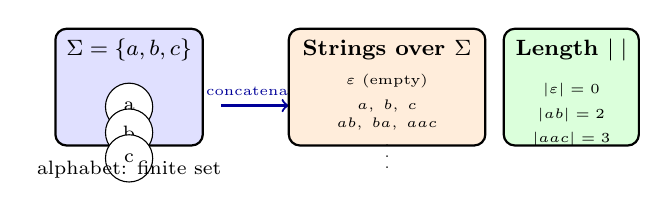
\begin{tikzpicture}[scale=0.78,every node/.style={font=\scriptsize}]
\draw[thick,fill=blue!12,rounded corners=4pt] (-1.2,-0.5) rectangle (1.2,1.4);
\node[font=\footnotesize\bfseries] at (0,1.05) {$\Sigma=\{a,b,c\}$};
\foreach \i/\ch in {1/a,2/b,3/c} {\node[draw,circle,fill=white,minimum size=0.6cm] at (0,0.55-0.42*\i) {\ch};}
\node at (0,-0.9) {alphabet: finite set};
% arrow to strings
\draw[->,thick,blue!60!black] (1.5,0.15)--(2.6,0.15) node[midway,above,font=\tiny] {concatenate};
\begin{scope}[xshift=4.2cm]
\draw[thick,fill=orange!14,rounded corners=4pt] (-1.6,-0.5) rectangle (1.6,1.4);
\node[font=\footnotesize\bfseries] at (0,1.05) {Strings over $\Sigma$};
\node[font=\tiny] at (0,0.55) {$\varepsilon$ (empty)};
\node[font=\tiny] at (0,0.15) {$a,\;b,\;c$};
\node[font=\tiny] at (0,-0.15) {$ab,\;ba,\;aac$};
\node[font=\tiny] at (0,-0.55) {$\vdots$};
\end{scope}
\begin{scope}[xshift=7.2cm]
\draw[thick,fill=green!14,rounded corners=4pt] (-1.1,-0.5) rectangle (1.1,1.4);
\node[font=\footnotesize\bfseries] at (0,1.05) {Length $|\;|$};
\node[font=\tiny] at (0,0.4) {$|\varepsilon|=0$};
\node[font=\tiny] at (0,0.0) {$|ab|=2$};
\node[font=\tiny] at (0,-0.4) {$|aac|=3$};
\end{scope}
\end{tikzpicture}
\caption{Alphabet $\Sigma$ is a finite symbol set; strings are finite sequences over $\Sigma$; $|w|$ counts symbols.}
\label{fig:alphabet-strings}
\end{figure}

\begin{definition}[String, empty string, length]
A \emph{string} (word) over $\Sigma$ is a finite sequence $w=a_1a_2\cdots a_n$ with each $a_i\in\Sigma$, $n\ge0$. When $n=0$ we get the \emph{empty string} $\varepsilon$. The \emph{length} $|w|=n$.
\end{definition}
We write $\Sigma^*$ for ``all strings'' (defined formally below). $|\Sigma|=k$ means alphabet size $k$.

\begin{definition}[String operations]
For $x=a_1\cdots a_m$, $y=b_1\cdots b_n$: \emph{concatenation} $xy=a_1\cdots a_m b_1\cdots b_n$; \emph{reversal} $x^R=a_m\cdots a_1$ ($\varepsilon^R=\varepsilon$); $z$ is a \emph{substring} of $w$ if $w=xzy$ for some $x,y$; prefix / suffix are $x$ / $y$ when $y=\varepsilon$ / $x=\varepsilon$.
\end{definition}

\begin{example}[Laws by picture then proof]
$|xy|=|x|+|y|$, $(xy)z=x(yz)$, $\varepsilon w=w\varepsilon=w$, and $(w^R)^R=w$. Intuitively, concatenation glues two rows of symbols. Formally, $(xy)z$ and $x(yz)$ are the same symbol sequence $a_1\cdots a_m b_1\cdots b_n c_1\cdots c_p$. Hence concatenation is associative with identity $\varepsilon$---a monoid.
\end{example}

Counting: if $|\Sigma|=k$, there are $k^n$ strings of length $n$, and $\sum_{i=0}^{n}k^i$ of length $\le n$. For binary $\Sigma=\{0,1\}$, $2^n$ strings of length $n$---the familiar exponential. Thus even for $k=1$, say $\Sigma=\{a\}$, there is exactly one string per length: $\Sigma^*=\{\varepsilon,a,aa,\dots\}$ in bijection with $\mathbb{N}$ via $n\mapsto a^n$.
\begin{example}[Small enumeration]
Binary $\Sigma=\{0,1\}$ with shortlex: length $0$: $\varepsilon$ ($1$ string); length $1$: $0,1$ ($2$); length $2$: $00,01,10,11$ ($4$); length $\le2$: $7$ strings. In general $|\Sigma^{\le n}|=(k^{n+1}-1)/(k-1)$ for $k>1$ (geometric sum).
For $\Sigma=\{a,b,c\}$, $|\Sigma^{\le2}|=1+3+9=13$.
\end{example}

% TikZ 2: concatenation as gluing bars
\begin{figure}[h]
\centering
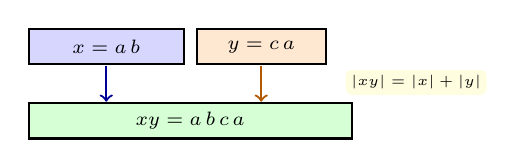
\begin{tikzpicture}[scale=0.82,every node/.style={font=\scriptsize}]
\draw[thick,fill=blue!16] (0,0) rectangle (2.4,0.55);
\node at (1.2,0.27) {$x=a\,b$};
\draw[thick,fill=orange!18] (2.6,0) rectangle (4.6,0.55);
\node at (3.6,0.27) {$y=c\,a$};
\draw[thick,fill=green!16] (0,-1.15) rectangle (5.0, -0.60);
\node at (2.5,-0.87) {$xy=a\,b\,c\,a$};
\draw[->,thick,blue!60!black] (1.2,-0.02)--(1.2,-0.58);
\draw[->,thick,orange!70!black] (3.6,-0.02)--(3.6,-0.58);
\node[font=\tiny,fill=yellow!12,rounded corners=2pt,inner sep=2pt] at (6.0,-0.28) {$|xy|=|x|+|y|$};
\end{tikzpicture}
\caption{Concatenation glues symbol rows; length adds; $\varepsilon$ is the empty row.}
\label{fig:concat-bar}
\end{figure}

% ============================================================
\section{Languages: Sets of Strings}
\label{sec:languages}
A \emph{language} over $\Sigma$ is any set $L\subseteq\Sigma^*$---finite or infinite. This set viewpoint lets us reuse Boolean operations.

\begin{definition}[Language operations]
For $L,L_1,L_2\subseteq\Sigma^*$: complement $\overline{L}=\Sigma^*\setminus L$; union $L_1\cup L_2$, intersection $L_1\cap L_2$; concatenation $L_1L_2=\{xy\mid x\in L_1,\,y\in L_2\}$; $L^R=\{w^R\mid w\in L\}$; power $L^0=\{\varepsilon\}$, $L^{n+1}=L^nL$.
\end{definition}

\begin{example}[Finite vs.\ infinite]
Over $\Sigma=\{0,1\}$: $L_1=\{01,10\}$ (finite, $|L_1|=2$); $L_2=\{0^n1^n\mid n\ge0\}=\{\varepsilon,01,0011,\dots\}$ (infinite, one string per $n$); $L_3=\Sigma^*$ (all strings); $L_4=\emptyset$ (no strings) vs.\ $\{\varepsilon\}$ (one string, the empty one)---a classic confusion.
\end{example}

\begin{remark}[Empty confusion]
$\emptyset\neq\{\varepsilon\}$: the first has $0$ strings, the second has $1$. Moreover $\emptyset L=\emptyset$ but $\{\varepsilon\}L=L$. Concatenating ``no choice'' yields no word; concatenating ``choose nothing'' leaves $L$ unchanged.
\end{remark}

% TikZ 3: Venn for language operations
\begin{figure}[h]
\centering
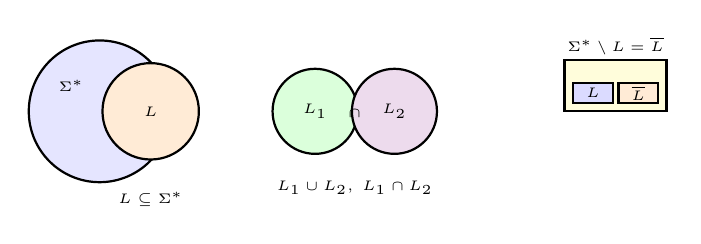
\begin{tikzpicture}[scale=0.72,every node/.style={font=\scriptsize}]
\begin{scope}
\draw[thick,fill=blue!10] (0,0) circle (1.25);
\draw[thick,fill=orange!16] (0.9,0) circle (0.85);
\node[font=\tiny] at (-0.5,0.45) {$\Sigma^*$};
\node[font=\tiny] at (0.9,0) {$L$};
\node[font=\tiny] at (0.9,-1.55) {$L\subseteq\Sigma^*$};
\end{scope}
\begin{scope}[xshift=4.5cm]
\draw[thick,fill=green!14] (-0.7,0) circle (0.75);
\draw[thick,fill=violet!14] (0.7,0) circle (0.75);
\node[font=\tiny] at (-0.7,0) {$L_1$};
\node[font=\tiny] at (0.7,0) {$L_2$};
\node[font=\tiny] at (0,-0.05) {\tiny $\cap$};
\node[font=\tiny] at (0,-1.35) {$L_1\cup L_2,\;L_1\cap L_2$};
\end{scope}
\begin{scope}[xshift=8.2cm]
\draw[thick,fill=yellow!14] (0,0) rectangle (1.8,0.9);
\draw[thick,fill=blue!14] (0.15,0.15) rectangle (0.85,0.50);
\draw[thick,fill=orange!16] (0.95,0.15) rectangle (1.65,0.50);
\node[font=\tiny] at (0.9,1.15) {$\Sigma^*\setminus L=\overline{L}$};
\node[font=\tiny] at (0.5,0.32) {$L$};
\node[font=\tiny] at (1.30,0.32) {$\overline{L}$};
\end{scope}
\end{tikzpicture}
\caption{Languages sit inside $\Sigma^*$; Boolean operations are set operations; complement is relative to $\Sigma^*$.}
\label{fig:lang-venn}
\end{figure}

% ============================================================
\section{Kleene Star and Closure}
\label{sec:kleene}
We close a language under concatenation repeatedly.

\begin{definition}[Kleene star and plus]
$L^*=\bigcup_{n\ge0}L^n=\{\varepsilon\}\cup L\cup LL\cup LLL\cup\cdots$. $L^+=LL^*=L^*L=\bigcup_{n\ge1}L^n=L^*\setminus\{\varepsilon\}$ if $\varepsilon\notin L$; in general $L^*=L^+\cup\{\varepsilon\}$. $\Sigma^*$ is the special case $L=\Sigma$ viewed as $|\Sigma|$ one-symbol strings.
\end{definition}

Intuition: $L^*$ is ``zero or more $L$-blocks glued''; $L^+$ is ``one or more''. For $L=\{a\}$: $L^*=\{\varepsilon,a,aa,aaa,\dots\}=a^*$ in regex notation; $(L^*)^*=L^*$ (idempotent).

\begin{theorem}[Algebraic laws]
For all $L$: $(L^*)^*=L^*$, $\emptyset^*=\{\varepsilon\}$, $\{\varepsilon\}^*=\{\varepsilon\}$, and $L^*\supseteq L$. If $L_1\subseteq L_2$ then $L_1^*\subseteq L_2^*$. However $(L_1\cup L_2)^*\neq L_1^*\cup L_2^*$ in general.
\end{theorem}
\begin{proof}
$(L^*)^*$ concatenates blocks each itself a concatenation of $L$-blocks---still a concatenation of $L$-blocks. Counterexample for union: $L_1=\{a\},L_2=\{b\}$ gives $ab\in(L_1\cup L_2)^*$ but $ab\notin L_1^*\cup L_2^*=\{a\}^*\cup\{b\}^*$. \qed
\end{proof}

\begin{example}[Counting $\Sigma^*$]
$|\Sigma^n|=|\Sigma|^n$. Hence $\Sigma^*$ is countably infinite and enumerable in \emph{shortlex} (by length then dictionary): $\varepsilon,0,1,00,01,10,11,000,\dots$ for binary. Lexicographic alone is not a well-order for listing $\Sigma^*$ without grouping by length.
\end{example}

% ============================================================
\section{Orderings and Cardinality of Languages}
\label{sec:ordering}
\emph{Intuition:} list all strings shortest first; within each length, dictionary order. This \emph{shortlex} is the canonical enumeration that proves $\Sigma^*$ is countable---crucial for diagonalisation in Ch.~7.

\begin{definition}[Lexicographic vs.\ shortlex]
Fix an order on $\Sigma$ (e.g.\ $0<1$). \emph{Lexicographic} ($\le_{\rm lex}$) compares at the first differing position (and $\varepsilon$ is smallest; a prefix is smaller than its extension). \emph{Shortlex} ($\le_{\rm sl}$): $x\le_{\rm sl}y$ if $|x|<|y|$ or $|x|=|y|$ and $x\le_{\rm lex}y$.
\end{definition}

\begin{theorem}[Countability]
For finite $\Sigma$, $\Sigma^*$ is countable; the set of all languages $\mathcal{P}(\Sigma^*)$ is uncountable. Shortlex gives an explicit bijection $\Sigma^*\to\mathbb{N}$.
\end{theorem}
\begin{proof}
Shortlex lists strings by increasing length; each length class has $k^n$ strings ($k=|\Sigma|$), finite, so every string appears at a finite position---a bijection $f(w)=$ rank in shortlex. Uncountability of $\mathcal{P}(\Sigma^*)$ follows from Cantor: if $\Sigma^*$ were countable, its power set would be strictly larger, i.e.\ $|\mathcal{P}(\mathbb{N})|>|\mathbb{N}|$. \qed
\end{proof}

\begin{example}[Why shortlex not plain lex?]
Plain lex on $\{0,1\}^*$ gives $\varepsilon<0<00<000<\cdots$---infinitely many strings before $1$, so $1$ has no finite rank.
Shortlex avoids this by finishing each length:
\begin{center}
$\varepsilon$ ($0$ of len $0$);\quad $0,1$ ($2$ of len $1$);\quad $00,01,10,11$ ($4$ of len $2$);\quad $\dots$
\end{center}
\end{example}

% ============================================================
\section{Chapter Notes}
Finite alphabets, strings, and Kleene closure were formalised by Kleene (1956) and systematised by Hopcroft--Ullman. The $\emptyset$ vs.\ $\{\varepsilon\}$ pitfall recurs in every later chapter; test it whenever a construction claims ``no word''. Shortlex enumeration underlies dovetailing in Ch.~6--7 and the existence of non-recursively-enumerable languages.

% ============================================================
\section{Exercises}
\label{sec:ch01-exercises}
\begin{enumerate}[label=E1.\arabic*, leftmargin=*, itemsep=0.8em]
\item \textbf{Empty vs.\ empty language.} Give $\Sigma$, then compute $|\{\varepsilon\}|$, $|\emptyset|$, $|\{\varepsilon\}^*|$, $|\emptyset^*|$, and $\emptyset\{a,b\}^*$. Explain why $\emptyset L=\emptyset\neq L$ in words.
\item \textbf{Counting.} For $\Sigma=\{a,b,c\}$ count strings of length exactly $3$ and $\le3$. Prove $|\Sigma^n|=|\Sigma|^n$ by induction on $n$, using $|\Sigma^{n+1}|=|\Sigma|\cdot|\Sigma^n|$.
\item \textbf{Star laws.} Prove $(L^*)^*=L^*$ and find $L_1,L_2$ with $(L_1L_2)^*\neq L_1^*L_2^*$. Prove or disprove: $(L^R)^*=(L^*)^R$.
\item \textbf{Reversal.} Prove $(xy)^R=y^Rx^R$ and by induction that $(w^n)^R=(w^R)^n$, then deduce $(L^n)^R=(L^R)^n$ and the previous exercise.
\item \textbf{Lexicographic pathology.} List $\Sigma^*=\{0,1\}^*$ first in lexicographic ($0<1$) order: $\varepsilon,0,00,000,\dots$. Why does $1$ never appear? Define shortlex and prove it enumerates $\Sigma^*$ as $\mathbb{N}$.
\end{enumerate}
% End of Chapter 1
